%----------------------------------------------------------------------------------------
%	SECTION 1
%----------------------------------------------------------------------------------------

\section{Science and Mathematics (SM)}

\subsection*{SM1(i, b, m)}

Multiple courses (mainly from years 2 and 3) have contributed to my knowledge and understanding of scientific principles and methodology necessary to underpin my education in Architectural Engineering.
A main contributor was \textit{Thermal Performance Studies}.
On this course I learned the scientific principles of psychrometrics, i.e. the properties of air-vapour mixtures (especially/ like air), and how to use this knowledge in the design of air conditioners, heat exchangers and cooling towers.
Learning about the environmental effects of refrigerants has contributed to my understanding of the evolution of air conditioners, from using carbon- and fluoride-based refrigerants to water and eventually phase change materials (PCMs) like Sunamp uses.

Learning the scientific principles of related disciplines has helped me enrich my appreciation of the scientific and engineering context of my discipline.
\textit{Statistics for Science} has, for example, helped me understand the proper methodology behind sampling populations and to identify bias in data.
\textit{Hydraulics and Hydrology A}, a civil engineering course, helped me appreciate the hydrological cycle (relevant to rainwater and urban drainage) and water flow in pipes (relevant to drainage, water supply and heating systems).


\subsection*{SM2(i, b, m)}

\textit{Mathematics for Engineers and Scientists 1 and 2} and \textit{Statistics for Science} all further developed my knowledge and understanding of mathematical and statistical methods.
I have been able to apply this knowledge in the analysis and solution of engineering problems.
For example, I used it to work out the yield of an array of photovoltaic panels (PV) in \textit{Energy and Buildings} as well as the yield of a set of turbines in a tidal energy generation system as part of my group project in \textit{Design Project}.


\subsection*{SM3(b, m)}

Other engineering disciplines that I have gained knowledge and understanding from are predominantly civil and structural.
These were acquired through the following courses: \textit{Mechanics B}, \textit{Construction Technology 1 and 2},  and \textit{Hydraulics and Hydrology A}.
%\hl{I cannot remember how I have applied or integrated this knowledge though...
%pipes?
%materials choice?}
I have been able to apply and integrate this knowledge and understanding to support study of my own engineering discipline, Architectural Engineering.
For example, during a \hl{CFD (1st time I mention CFD?)} modelling exercise in Laboratory Project, I was able to identify laminar and turbulent flows, something I had learned about it in \textit{Hydraulics and Hydrology A}.
This enabled me to refine and improve my CFD model.


\subsection*{SM4m}

A range of courses increased my awareness of developing technologies relevant to Architectural Engineering and building services.
In \textit{Building Services Technology}, \textit{Energy and Buildings}, \textit{Dissertation} and \textit{Innovation in Construction Practice}, I respectively learned about technologies such as modern windcatchers, smart meters, Building Information Modelling (BIM) and virtual and augmented reality.
I was also exposed to a developing technology during my placement at Sunamp: their heat batteries.
\hl{refer to work done at Sunamp?}


\subsection*{SM5m}

\hl{Is this skill about software???}
\textit{Design Software Applications} and \textit{Laboratory Project} enabled me to gain a comprehensive knowledge and understanding of software used by architectural engineers.
I learned how steady-state and dynamic software applications function, was made aware of the mathematical \hl{models/ formulas} they are based on and learned about their limitations.
\hl{Should I give examples of limitations to demonstrate my knowledge/ understanding? Not necessarily part of marking criteria.}
I was introduced to and got to practise using the following applications:
\begin{itemize}
    \item Steady-state: iSBEM (an interface for Simplified Building Energy Model), SAP (Standard Assessment Procedure) and PHOENICS (a CFD software application)
    \item Dynamic: IES-VE (Integrated Environmental Solutions - Virtual Environment)
    \item Computational fluid dynamics (CFD): PHOENICS?
\end{itemize}

% Please add the following required packages to your document preamble:
% \usepackage{booktabs}
\begin{table}[htbp]
\begin{tabular}{@{}lp{8cm}@{}}
\toprule
Type of software & Applications \\ \midrule
Steady-state & iSBEM (an interface for Simplified Building Energy Model) \\
 & SAP (Standard Assessment Procedure) \\
 & PHOENICS (a CFD software application) \\
Dynamic & IES-VE (Integrated Environmental Solutions - Virtual Environment) \\
Computational fluid dynamics (CFD)? & PHOENICS? \\ \bottomrule
\end{tabular}
\end{table}

\hl{List or table?}

\hl{Although it is outside the scope of this learning outcome, I would like to add that these courses did not allow me to properly develop my skills in using the software...}


\subsection*{SM6m}

\hl{How does this fall under Science and Maths heading?}

I have been able to critically evaluate and apply a range of concepts, including some outside engineering, in my engineering projects.
\hl{EXAMPLE 1:}
I learned about the sustainable design hierarchy (see Figure~\ref{fig_hierarchy}) during my placement at Arup.
I then applied this approach to the design of a library for a group project in \textit{Critical Architectural Studies}, helping us earn the first prize in Sustainable Design (see Figure~\ref{fig_award}).
\hl{EXAMPLE 2:}
Upon conducting a post-occupancy evaluation (POE) for \textit{Environment and Behaviour}, I came across a social sciences journal paper about survey research.
It analysed typical response styles and suggested how to design questionnaires to avoid biased or inaccurate data collection.
Using these \hl{criteria/ suggestions}, I was able to critically evaluate the success of the questionnaire used for the POE in \textit{Environment and Behaviour} and design an improved survey questionnaire for the acoustic \textit{Laboratory Project}.

\begin{figure}[htbp]
	\centering
	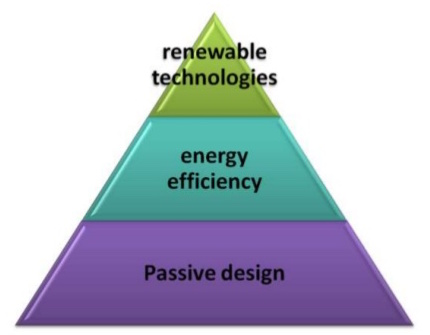
\includegraphics[width=10cm]{figures/Hierarchy.jpg}
	\rule{\textwidth}{0.5pt} % use line???
	\caption{The sustainable design hierarchy \citep{Dougherty:online}.}
	\label{fig_hierarchy}
\end{figure}


\begin{figure}[htbp]
	\centering
	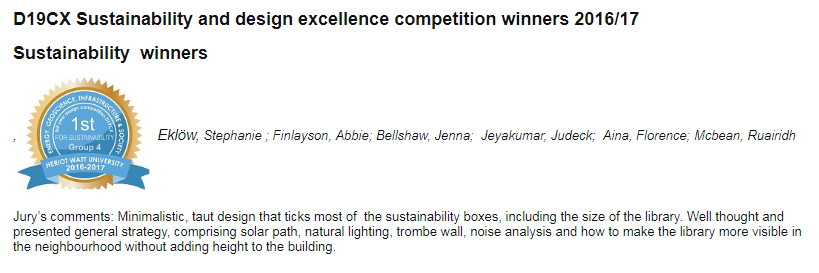
\includegraphics[width=\textwidth]{figures/SustainabilityAward.png}
	\rule{\textwidth}{0.5pt} % use line???
	\caption{First prize for sustainability awarded to my group for our library design in \textit{Critical Architectural Studies} (D19CX).}
	\label{fig_award}
\end{figure}

\hl{Other courses?}
\begin{itemize}
	\item Use of solar gain in pool house (\textit{first year collaborative project})?
	\item Contact factor in \textit{LAB CFD}?
	\item Learned in \textit{CAS}, applied again in \textit{y4 collab}: make design concept red thread...
\end{itemize}


